
\label{sec:ergebnisse}

Sämtliche Performance-Ergebnisse sind rein GPU-limitiert, daher seien hier nur die
Graphikkarten vorgestellt, mit denen \emph{Flewnit} getestet wurde :

Nvidia Geforce GT 435M 
	\footnote{http://www.nvidia.com/object/product-geforce-gt-435m-us.html} - GPU, eine
	Mittelklasse-Notebook-Graphikkarte der \emph{Fermi}-Architektur mit 1 GB RAM,
	2 Compute Units zu je 48 Recheneinheiten, in CUDA-Terminologie auch "`CUDA-Cores"' genannt.

\subsection{Visuelles Rendering}

	Zunächst sollen die Ergebnisse ohne die mechanische Simulationsdömane, also die Fluid-Simulation
	vorgestellt werden.
	Sämtliche Non-OpenCl- Benchmarks wurden nur auf der auf einer 
	

\begin{figure}[!h]

	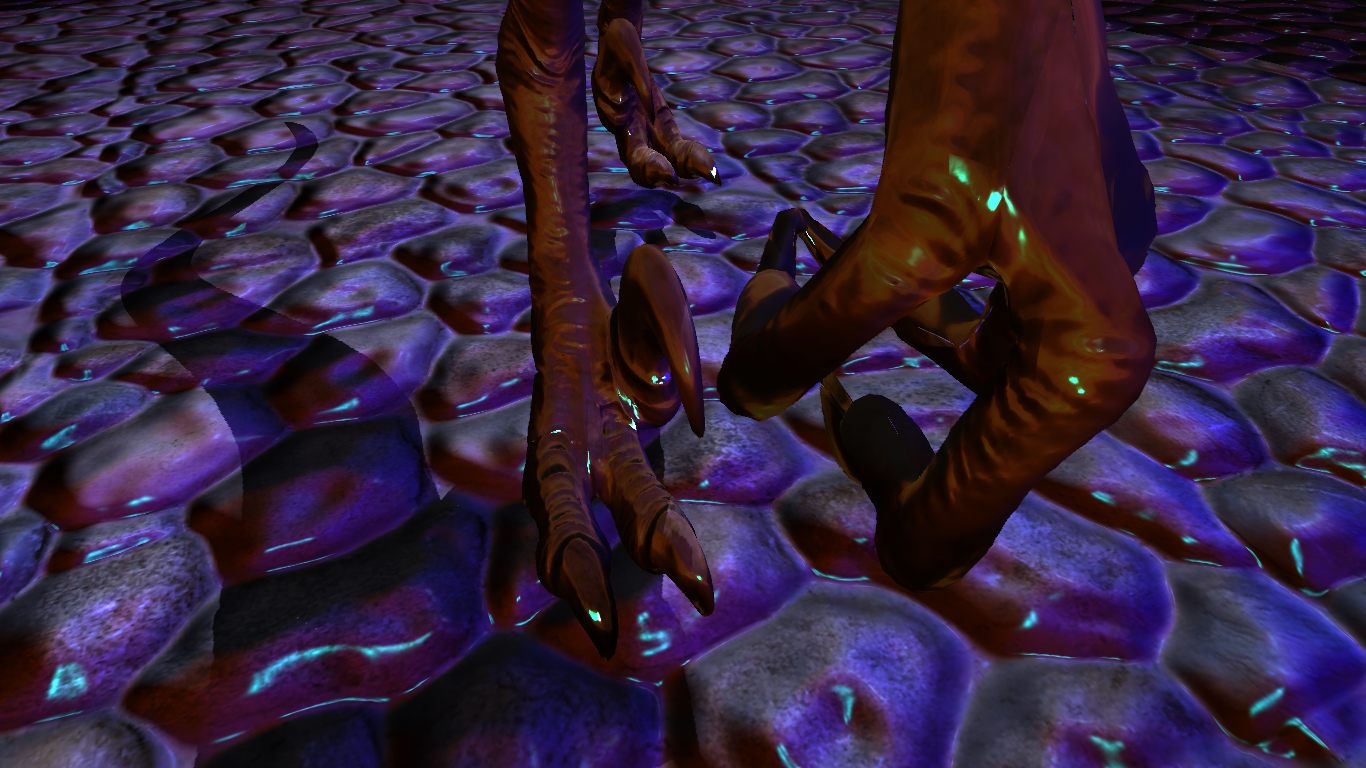
\includegraphics[width=1.2\textwidth]{Screenshot_raptorExtremities_allFX.png} 
	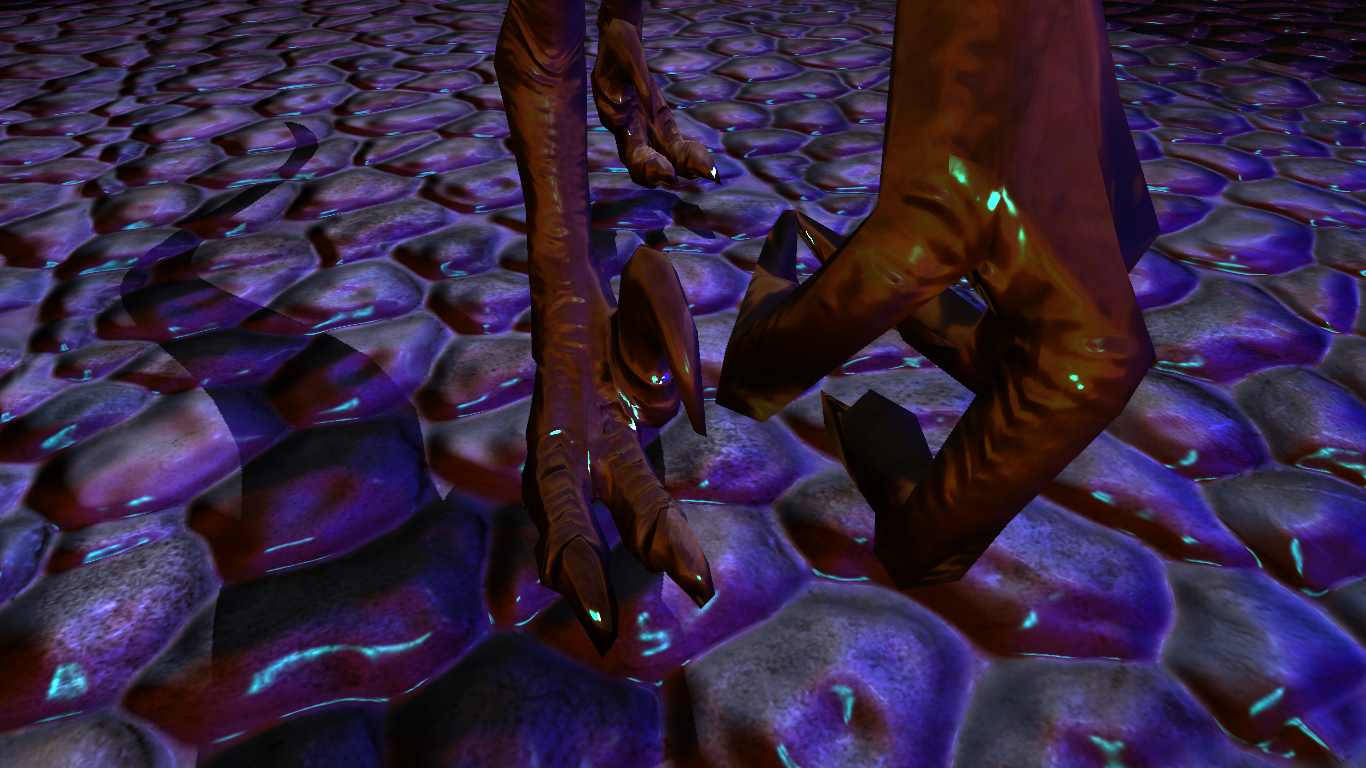
\includegraphics[width=1.2\textwidth]{Screenshot_raptorExtremities_allFX_withoutTess.png}

	\caption{Die Extremitäten des Raptor-modells; Oben: tesseliert, texturiert, normal mapped, environment mapped, 
	beleuchtet von fünf Lichtquellen , shadow mapped von einer Lichtquelle; Unten: wie oben, nur ohne Tessellation
	}
	\label{fig:raptorExtremitiesTessVSNonTess}
\end{figure}

	Abb. \ref{fig:raptorExtremitiesTessVSNonTess} zight die Komponenten des Raptor-Modells, die vom
	zusätzlichen Geometrie-Detail besonders profitieren, nämlich die filigranen Extremitäten.
	Alle zur Zeit funktionsfähigen Shading-Features waren an diesen Renderings beteiligt



\begin{figure}[!h]	 	
	\begin{tabular}{ x{0.5\textwidth} x{0.5\textwidth} }
		
		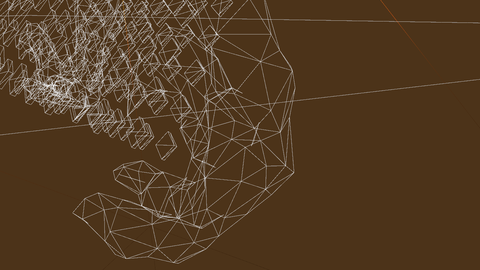
\includegraphics[width=0.5\textwidth]{resized/resized_Screenshot_raptorClaws_pure_WIRE.png} 
		wire frame	
		&
		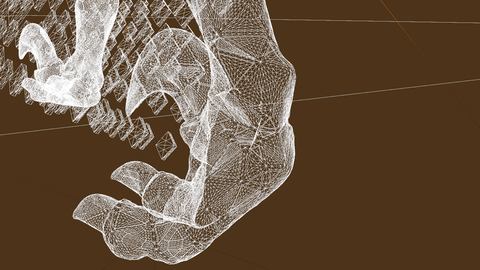
\includegraphics[width=0.5\textwidth]{resized/resized_Screenshot_raptorClaws_pure_WIRE_tess.png} 
		wire frame, tessellated
		\tabularnewline

		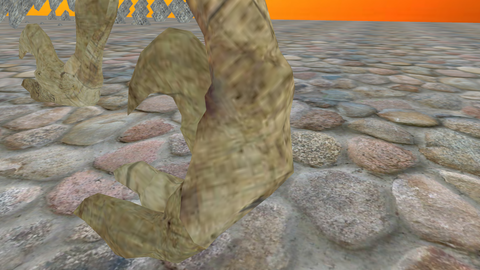
\includegraphics[width=0.5\textwidth]{resized/resized_Screenshot_raptorClaws_diffuseTex.png} 
		diffuse textured
		&
		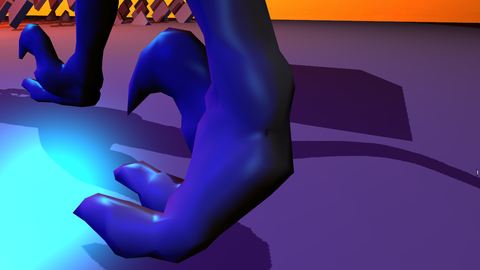
\includegraphics[width=0.5\textwidth]{resized/resized_Screenshot_raptorClaws_lighting.png}
		lighted
		\tabularnewline
		
		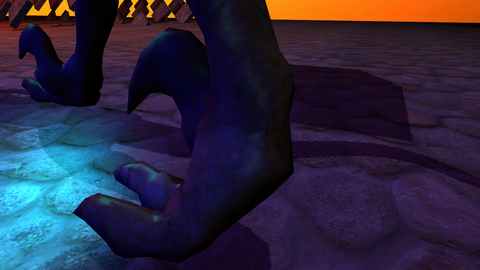
\includegraphics[width=0.5\textwidth]{resized/resized_Screenshot_raptorClaws_lighting_diffuseTex.png} 	
		lighted, diffuse textured
		&
		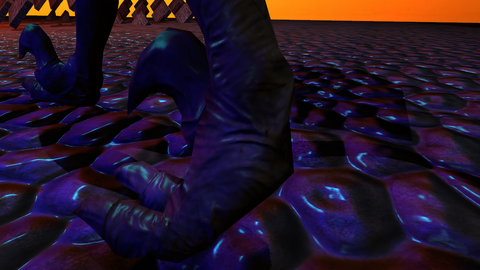
\includegraphics[width=0.5\textwidth]{resized/resized_Screenshot_raptorClaws_lighting_diffuseTex_normalMap.png}	
		lighted, diffuse textured, normal mapped
		\tabularnewline

		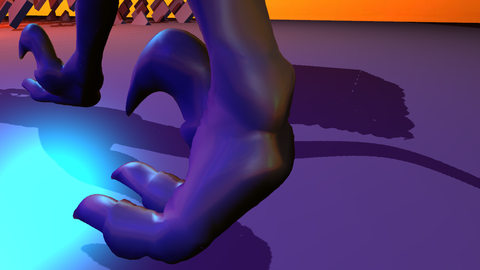
\includegraphics[width=0.5\textwidth]{resized/resized_Screenshot_raptorClaws_lighting_envmap_tess.png} 	
		lighted, diffuse textured, environment mapped, tessellated
		&
		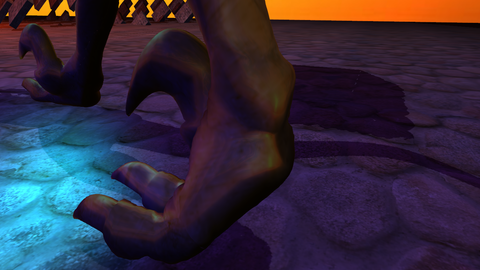
\includegraphics[width=0.5\textwidth]{resized/resized_Screenshot_raptorClaws_lighting_diffuseTex_envmap_tess.png}
		lighted, diffuse textured, environment mapped, tessellated
		\tabularnewline		
		
		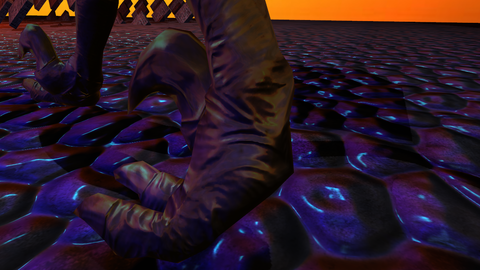
\includegraphics[width=0.5\textwidth]
			{resized/resized_Screenshot_raptorClaws_lighting_diffuseTex_normalMap_envMap.png} 	
		lighted, diffuse textured, normal mapped, environment mapped
		&
		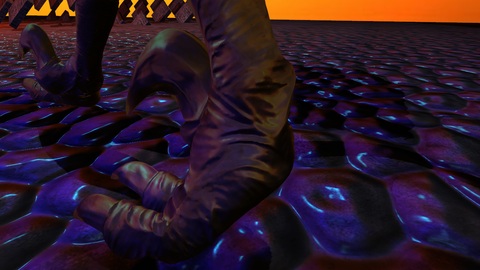
\includegraphics[width=0.5\textwidth]
			{resized/resized_Screenshot_raptorClaws_lighting_diffuseTex_normalMap_envMap_tess.png}		
		lighted, diffuse textured, normal mapped, environment mapped, tessellated
		\tabularnewline
	\end{tabular}
	\caption{Füße des Raptor-Modells, mit verschiedenen Permutationen aktivierter Shader-Features}
	\label{fig:shaderfeaturePermutations}
\end{figure}




\begin{figure}[!h]	 	
	\begin{tabular}{ x{0.5\textwidth} x{0.5\textwidth} }

   		\multicolumn{2}{ x{\textwidth} }{   			
    			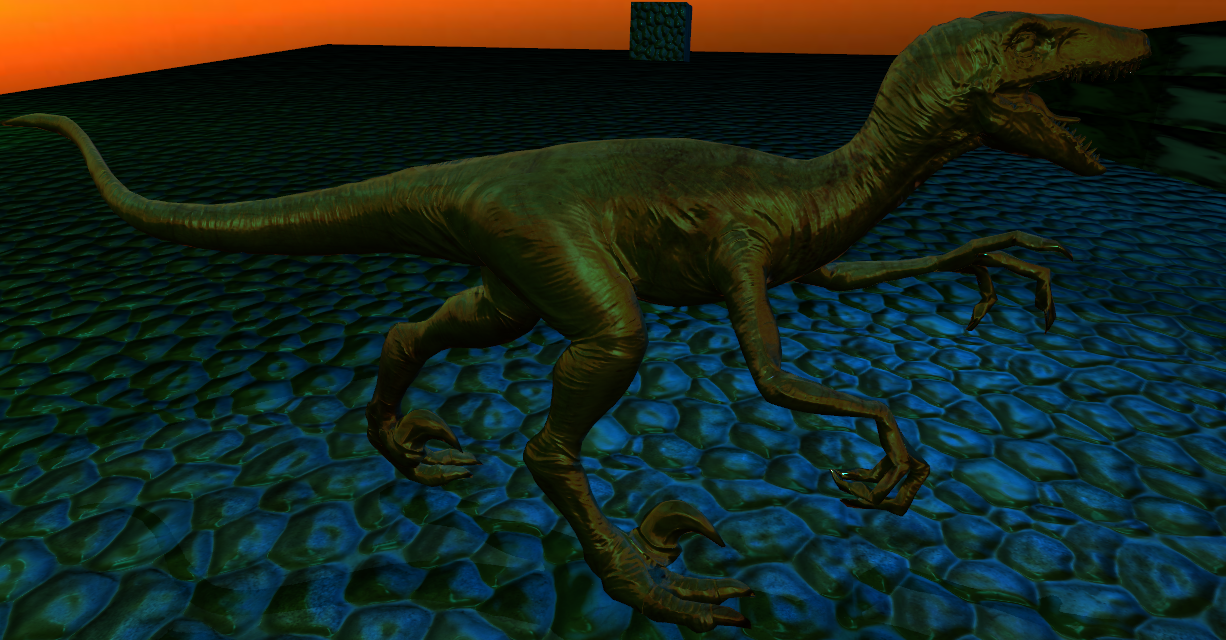
\includegraphics[width=\textwidth]{Screenshot_raptor_full.png} 
   		}	
   		\tabularnewline	
   		
   		\multicolumn{2}{ x{\textwidth} }{
    			Auf die Entfernung reicht das Normal Mapping noch aus,
		}
		\tabularnewline   		
		\multicolumn{2}{ x{\textwidth} }{
    			um Geometrie-Detail zu suggerieren ...
		}
		\tabularnewline
		
		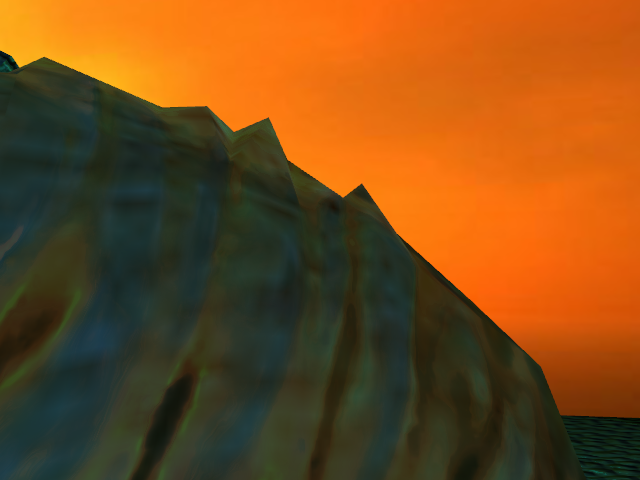
\includegraphics[width=0.4\textwidth]{Screenshot_raptorNeck_normal.png} 
		&
		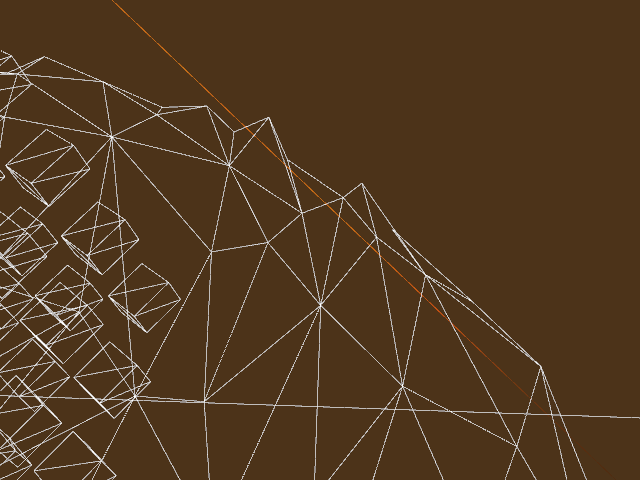
\includegraphics[width=0.4\textwidth]{Screenshot_raptorNeck_WIRE.png} 
		\tabularnewline
		
		\multicolumn{2}{ x{\textwidth} }{
			\multirow{1}{*}{
			... hier jedoch nicht mehr
			}
		}
		\tabularnewline
		
		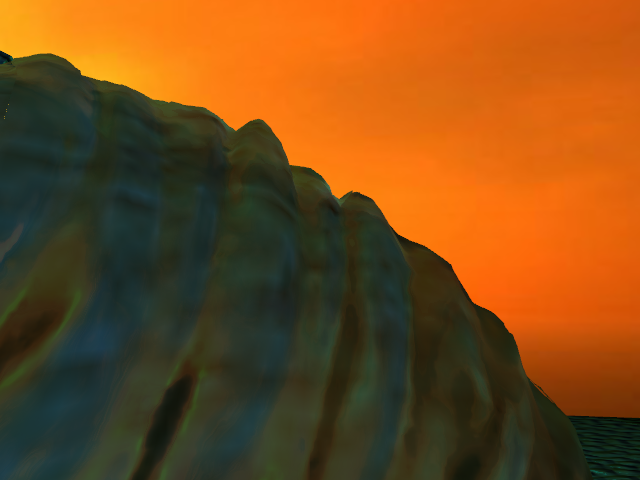
\includegraphics[width=0.4\textwidth]{Screenshot_raptorNeck_normaltess.png}
		&
		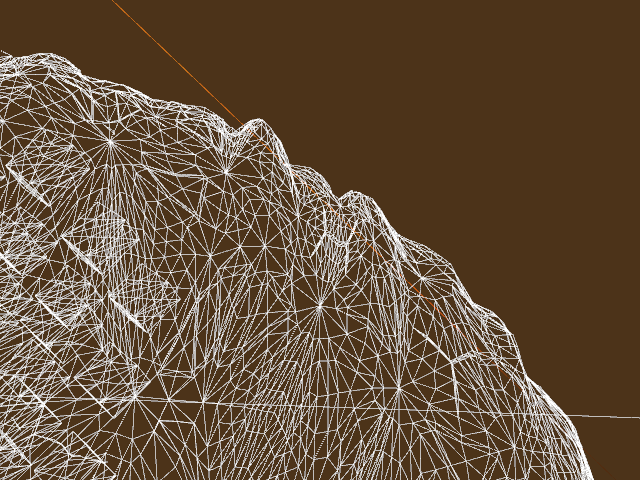
\includegraphics[width=0.4\textwidth]{Screenshot_raptorNeck_WIRE_tess.png}
		\tabularnewline

		%------------------------------------------------------------------------------
			
		%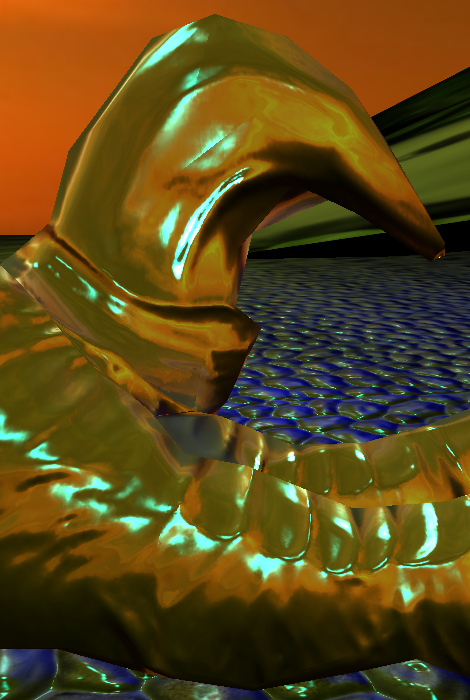
\includegraphics[width=0.4\textwidth]{Screenshot_raptorFootCloseUp_nonTess.png}
		%&
		%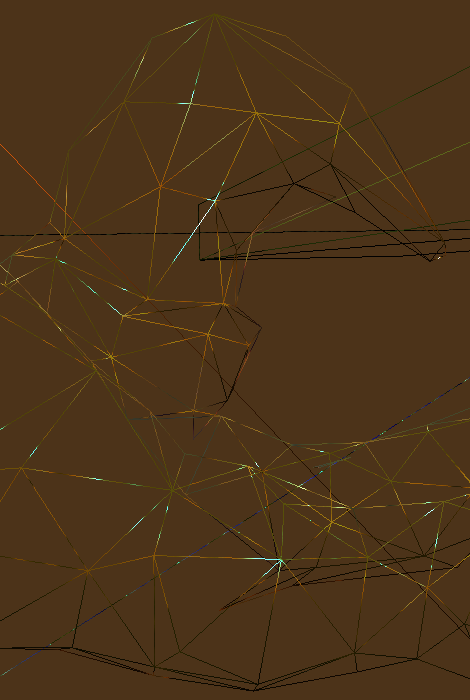
\includegraphics[width=0.4\textwidth]{Screenshot_raptorFootCloseUp_WIRE_nonTess.png}
		%\tabularnewline
		
		%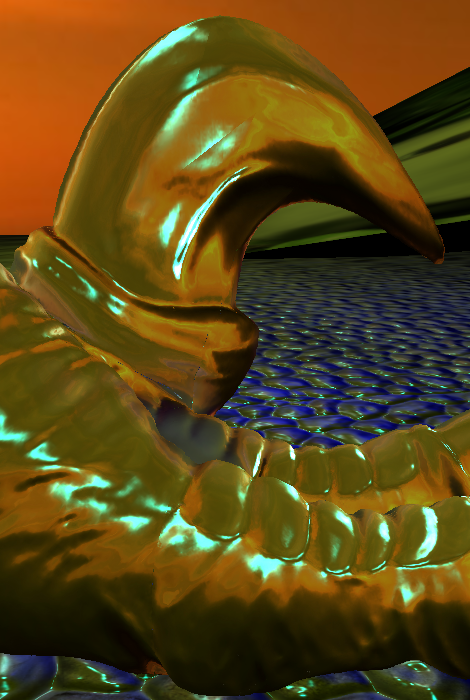
\includegraphics[width=0.4\textwidth]{Screenshot_raptorFootCloseUp_tess.png}
		%&
		%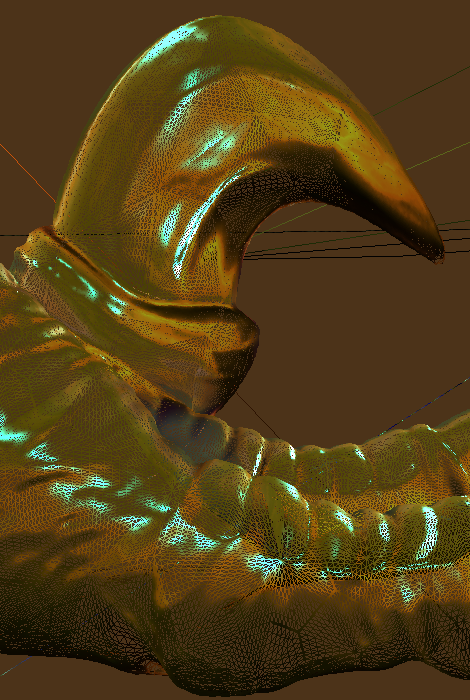
\includegraphics[width=0.4\textwidth]{Screenshot_raptorFootCloseUp_WIRE_tess.png}
		%\tabularnewline

	\end{tabular}
	\caption{Gegenüberstellung des Detail-Grades mit und ohne Tessellation, Teil 1}
	\label{fig:sefef}
\end{figure}

\begin{figure}[!h]	 	
	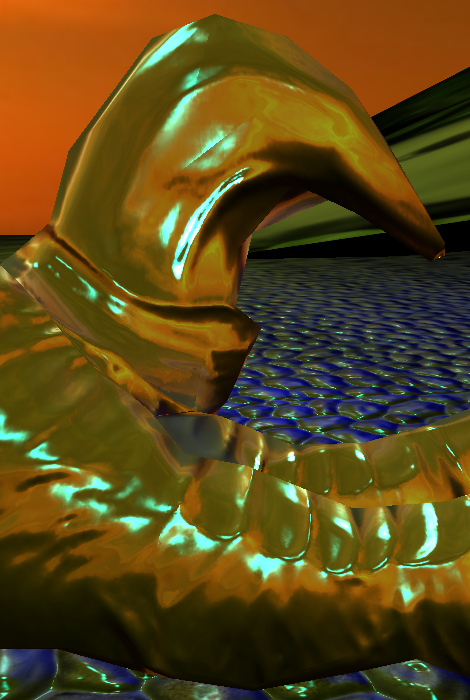
\includegraphics[width=0.5\textwidth]{Screenshot_raptorFootCloseUp_nonTess.png} 
	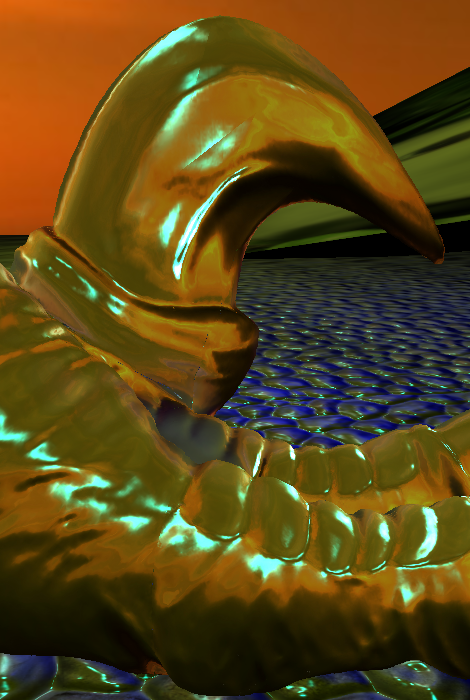
\includegraphics[width=0.5\textwidth]{Screenshot_raptorFootCloseUp_tess.png} 
	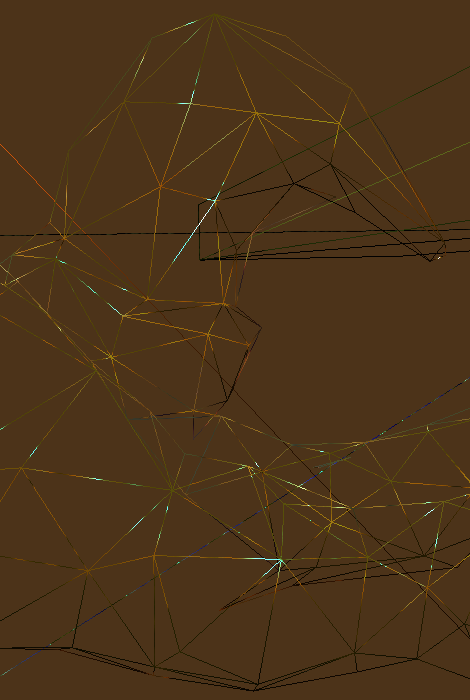
\includegraphics[width=0.5\textwidth]{Screenshot_raptorFootCloseUp_WIRE_nonTess.png} 
	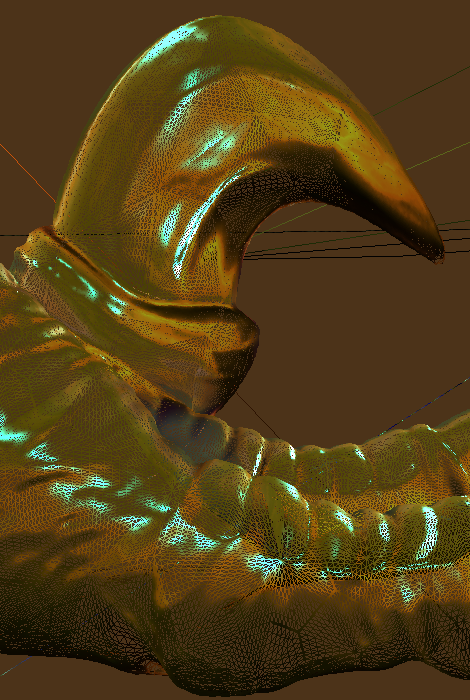
\includegraphics[width=0.5\textwidth]{Screenshot_raptorFootCloseUp_WIRE_tess.png} 

	\caption{Gegenüberstellung des Detail-Grades mit und ohne Tessellation, Teil 2}
	\label{fig:gegenueberstellungTessNonTess}
\end{figure}




\clearpage
